\documentclass[border=15pt, tikz]{standalone}
\usepackage[T1]{fontenc}
\usepackage[utf8]{inputenc}
\usepackage{tikz}
\usetikzlibrary{positioning, arrows.meta, decorations.pathreplacing, calc, fit}
\definecolor{clrattention}{HTML}{45B7D1}
\definecolor{clrattention_alt}{HTML}{96E6F0}
\definecolor{clrffn}{HTML}{F97068}
\definecolor{clrnorm}{HTML}{FFD93D}
\definecolor{clrembed}{HTML}{6BCB77}
\definecolor{clrresidual}{HTML}{4D96FF}
\definecolor{clroutput}{HTML}{C084FC}
\definecolor{clrspectral}{HTML}{22D3EE}
\definecolor{clrphysics}{HTML}{FB923C}
\definecolor{clrborder}{HTML}{334155}
\definecolor{clrtext}{HTML}{1E293B}
\definecolor{clrgroup_frame}{HTML}{94A3B8}
\definecolor{clrgroup_fill}{HTML}{F1F5F9}
\begin{document}
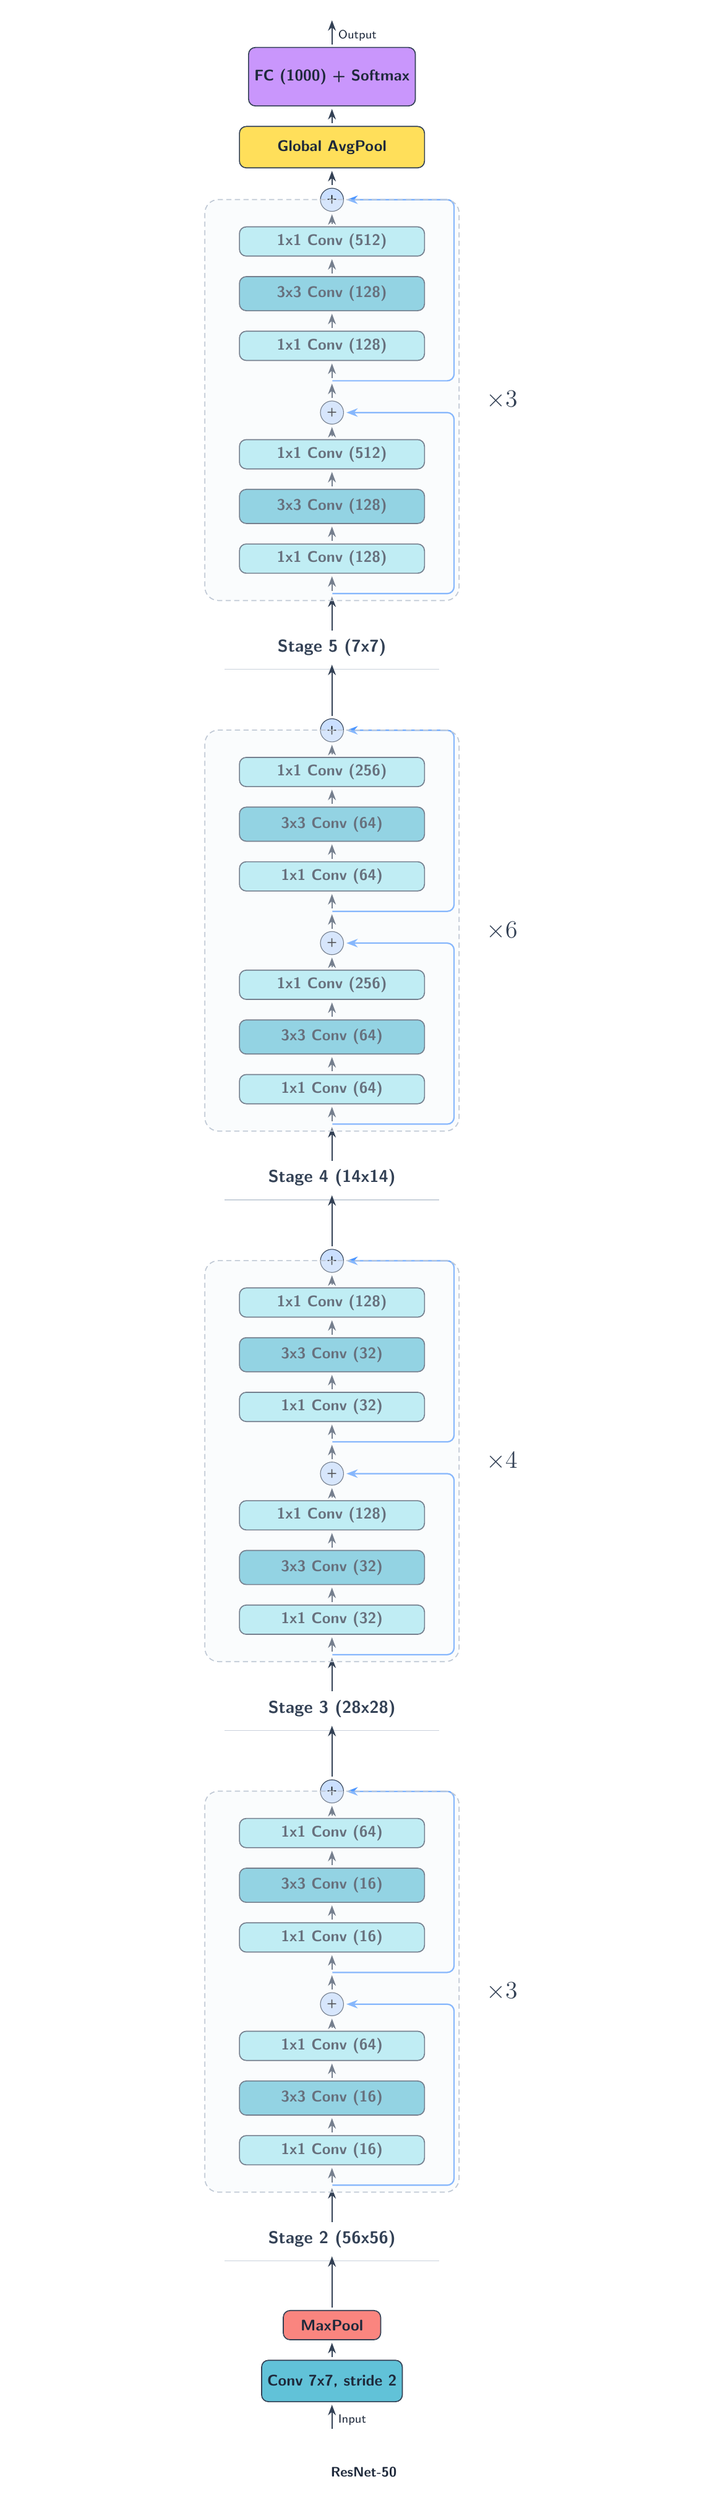
\begin{tikzpicture}[
    >=Stealth,
    every node/.style={font=\sffamily},
    block/.style={draw=clrborder, rounded corners=4pt, minimum width=3.8cm,
                  minimum height=0.85cm, font=\sffamily\small\bfseries,
                  text=clrtext, line width=0.6pt},
    arrow/.style={->, thick, color=clrborder, line width=0.7pt, shorten >=1.5pt, shorten <=1.5pt},
    skiparrow/.style={->, thick, color=clrresidual, line width=0.8pt, rounded corners=4pt, shorten >=1.5pt},
    label/.style={font=\sffamily\scriptsize, text=clrtext},
    subtitle/.style={font=\sffamily\footnotesize, text=clrtext},
]
\node[block, fill=clrattention!85, minimum width=1.87cm, minimum height=0.85cm, text=clrtext] (n_1) at (0,0) {Conv 7x7, stride 2};
\node[block, fill=clrffn!85, minimum width=2.0cm, minimum height=0.6cm, text=clrtext, above=0.4cm of n_1] (n_2) {MaxPool};
\node[inner sep=0, minimum height=0, above=1.0cm of n_2] (n_3_rule) {};
\draw[color=clrgroup_frame!50, line width=0.4pt] ([xshift=-2.2cm]n_3_rule.center) -- ([xshift=2.2cm]n_3_rule.center);
\node[above=4pt of n_3_rule, font=\sffamily\normalsize\bfseries, text=clrborder] (n_3) {Stage 2 (56x56)};
\node[inner sep=0, minimum size=0, above=0.8cm of n_3] (res_entry_4) {};
\node[block, fill=clrattention_alt!85, minimum width=3.8cm, minimum height=0.6cm, text=clrtext, above=0.4cm of res_entry_4] (n_5) {1x1 Conv (16)};
\node[block, fill=clrattention!85, minimum width=3.8cm, minimum height=0.7cm, text=clrtext, above=0.4cm of n_5] (n_6) {3x3 Conv (16)};
\node[block, fill=clrattention_alt!85, minimum width=3.8cm, minimum height=0.6cm, text=clrtext, above=0.4cm of n_6] (n_7) {1x1 Conv (64)};
\node[circle, draw=clrborder, fill=clrresidual!30, inner sep=2pt, font=\sffamily\scriptsize\bfseries, above=0.3cm of n_7] (add_8) {+};
\node[inner sep=0, minimum size=0, above=0.4cm of add_8] (res_entry_9) {};
\node[block, fill=clrattention_alt!85, minimum width=3.8cm, minimum height=0.6cm, text=clrtext, above=0.4cm of res_entry_9] (n_10) {1x1 Conv (16)};
\node[block, fill=clrattention!85, minimum width=3.8cm, minimum height=0.7cm, text=clrtext, above=0.4cm of n_10] (n_11) {3x3 Conv (16)};
\node[block, fill=clrattention_alt!85, minimum width=3.8cm, minimum height=0.6cm, text=clrtext, above=0.4cm of n_11] (n_12) {1x1 Conv (64)};
\node[circle, draw=clrborder, fill=clrresidual!30, inner sep=2pt, font=\sffamily\scriptsize\bfseries, above=0.3cm of n_12] (add_13) {+};
\node[inner sep=0, minimum height=0, above=1.0cm of add_13] (n_14_rule) {};
\draw[color=clrgroup_frame!50, line width=0.4pt] ([xshift=-2.2cm]n_14_rule.center) -- ([xshift=2.2cm]n_14_rule.center);
\node[above=4pt of n_14_rule, font=\sffamily\normalsize\bfseries, text=clrborder] (n_14) {Stage 3 (28x28)};
\node[inner sep=0, minimum size=0, above=0.8cm of n_14] (res_entry_15) {};
\node[block, fill=clrattention_alt!85, minimum width=3.8cm, minimum height=0.6cm, text=clrtext, above=0.4cm of res_entry_15] (n_16) {1x1 Conv (32)};
\node[block, fill=clrattention!85, minimum width=3.8cm, minimum height=0.7cm, text=clrtext, above=0.4cm of n_16] (n_17) {3x3 Conv (32)};
\node[block, fill=clrattention_alt!85, minimum width=3.8cm, minimum height=0.6cm, text=clrtext, above=0.4cm of n_17] (n_18) {1x1 Conv (128)};
\node[circle, draw=clrborder, fill=clrresidual!30, inner sep=2pt, font=\sffamily\scriptsize\bfseries, above=0.3cm of n_18] (add_19) {+};
\node[inner sep=0, minimum size=0, above=0.4cm of add_19] (res_entry_20) {};
\node[block, fill=clrattention_alt!85, minimum width=3.8cm, minimum height=0.6cm, text=clrtext, above=0.4cm of res_entry_20] (n_21) {1x1 Conv (32)};
\node[block, fill=clrattention!85, minimum width=3.8cm, minimum height=0.7cm, text=clrtext, above=0.4cm of n_21] (n_22) {3x3 Conv (32)};
\node[block, fill=clrattention_alt!85, minimum width=3.8cm, minimum height=0.6cm, text=clrtext, above=0.4cm of n_22] (n_23) {1x1 Conv (128)};
\node[circle, draw=clrborder, fill=clrresidual!30, inner sep=2pt, font=\sffamily\scriptsize\bfseries, above=0.3cm of n_23] (add_24) {+};
\node[inner sep=0, minimum height=0, above=1.0cm of add_24] (n_25_rule) {};
\draw[color=clrgroup_frame!50, line width=0.4pt] ([xshift=-2.2cm]n_25_rule.center) -- ([xshift=2.2cm]n_25_rule.center);
\node[above=4pt of n_25_rule, font=\sffamily\normalsize\bfseries, text=clrborder] (n_25) {Stage 4 (14x14)};
\node[inner sep=0, minimum size=0, above=0.8cm of n_25] (res_entry_26) {};
\node[block, fill=clrattention_alt!85, minimum width=3.8cm, minimum height=0.6cm, text=clrtext, above=0.4cm of res_entry_26] (n_27) {1x1 Conv (64)};
\node[block, fill=clrattention!85, minimum width=3.8cm, minimum height=0.7cm, text=clrtext, above=0.4cm of n_27] (n_28) {3x3 Conv (64)};
\node[block, fill=clrattention_alt!85, minimum width=3.8cm, minimum height=0.6cm, text=clrtext, above=0.4cm of n_28] (n_29) {1x1 Conv (256)};
\node[circle, draw=clrborder, fill=clrresidual!30, inner sep=2pt, font=\sffamily\scriptsize\bfseries, above=0.3cm of n_29] (add_30) {+};
\node[inner sep=0, minimum size=0, above=0.4cm of add_30] (res_entry_31) {};
\node[block, fill=clrattention_alt!85, minimum width=3.8cm, minimum height=0.6cm, text=clrtext, above=0.4cm of res_entry_31] (n_32) {1x1 Conv (64)};
\node[block, fill=clrattention!85, minimum width=3.8cm, minimum height=0.7cm, text=clrtext, above=0.4cm of n_32] (n_33) {3x3 Conv (64)};
\node[block, fill=clrattention_alt!85, minimum width=3.8cm, minimum height=0.6cm, text=clrtext, above=0.4cm of n_33] (n_34) {1x1 Conv (256)};
\node[circle, draw=clrborder, fill=clrresidual!30, inner sep=2pt, font=\sffamily\scriptsize\bfseries, above=0.3cm of n_34] (add_35) {+};
\node[inner sep=0, minimum height=0, above=1.0cm of add_35] (n_36_rule) {};
\draw[color=clrgroup_frame!50, line width=0.4pt] ([xshift=-2.2cm]n_36_rule.center) -- ([xshift=2.2cm]n_36_rule.center);
\node[above=4pt of n_36_rule, font=\sffamily\normalsize\bfseries, text=clrborder] (n_36) {Stage 5 (7x7)};
\node[inner sep=0, minimum size=0, above=0.8cm of n_36] (res_entry_37) {};
\node[block, fill=clrattention_alt!85, minimum width=3.8cm, minimum height=0.6cm, text=clrtext, above=0.4cm of res_entry_37] (n_38) {1x1 Conv (128)};
\node[block, fill=clrattention!85, minimum width=3.8cm, minimum height=0.7cm, text=clrtext, above=0.4cm of n_38] (n_39) {3x3 Conv (128)};
\node[block, fill=clrattention_alt!85, minimum width=3.8cm, minimum height=0.6cm, text=clrtext, above=0.4cm of n_39] (n_40) {1x1 Conv (512)};
\node[circle, draw=clrborder, fill=clrresidual!30, inner sep=2pt, font=\sffamily\scriptsize\bfseries, above=0.3cm of n_40] (add_41) {+};
\node[inner sep=0, minimum size=0, above=0.4cm of add_41] (res_entry_42) {};
\node[block, fill=clrattention_alt!85, minimum width=3.8cm, minimum height=0.6cm, text=clrtext, above=0.4cm of res_entry_42] (n_43) {1x1 Conv (128)};
\node[block, fill=clrattention!85, minimum width=3.8cm, minimum height=0.7cm, text=clrtext, above=0.4cm of n_43] (n_44) {3x3 Conv (128)};
\node[block, fill=clrattention_alt!85, minimum width=3.8cm, minimum height=0.6cm, text=clrtext, above=0.4cm of n_44] (n_45) {1x1 Conv (512)};
\node[circle, draw=clrborder, fill=clrresidual!30, inner sep=2pt, font=\sffamily\scriptsize\bfseries, above=0.3cm of n_45] (add_46) {+};
\node[block, fill=clrnorm!85, minimum width=3.8cm, minimum height=0.85cm, text=clrtext, above=0.4cm of add_46] (n_47) {Global AvgPool};
\node[block, fill=clroutput!85, minimum width=2.0cm, minimum height=1.2cm, text=clrtext, above=0.4cm of n_47] (n_48) {FC (1000) + Softmax};
\draw[arrow] (n_1.north) -- (n_2.south);
\draw[arrow] (n_2.north) -- (n_3.south);
\draw[arrow] (n_5.north) -- (n_6.south);
\draw[arrow] (n_6.north) -- (n_7.south);
\draw[arrow] (res_entry_4.north) -- (n_5.south);
\draw[arrow] (n_7.north) -- (add_8.south);
\draw[skiparrow] (res_entry_4.east) -- ++(2.5,0) |- (add_8.east);
\draw[arrow] (n_3.north) -- (res_entry_4.south);
\draw[arrow] (n_10.north) -- (n_11.south);
\draw[arrow] (n_11.north) -- (n_12.south);
\draw[arrow] (res_entry_9.north) -- (n_10.south);
\draw[arrow] (n_12.north) -- (add_13.south);
\draw[skiparrow] (res_entry_9.east) -- ++(2.5,0) |- (add_13.east);
\draw[arrow] (add_8.north) -- (res_entry_9.south);
\draw[arrow] (add_13.north) -- (n_14.south);
\draw[arrow] (n_16.north) -- (n_17.south);
\draw[arrow] (n_17.north) -- (n_18.south);
\draw[arrow] (res_entry_15.north) -- (n_16.south);
\draw[arrow] (n_18.north) -- (add_19.south);
\draw[skiparrow] (res_entry_15.east) -- ++(2.5,0) |- (add_19.east);
\draw[arrow] (n_14.north) -- (res_entry_15.south);
\draw[arrow] (n_21.north) -- (n_22.south);
\draw[arrow] (n_22.north) -- (n_23.south);
\draw[arrow] (res_entry_20.north) -- (n_21.south);
\draw[arrow] (n_23.north) -- (add_24.south);
\draw[skiparrow] (res_entry_20.east) -- ++(2.5,0) |- (add_24.east);
\draw[arrow] (add_19.north) -- (res_entry_20.south);
\draw[arrow] (add_24.north) -- (n_25.south);
\draw[arrow] (n_27.north) -- (n_28.south);
\draw[arrow] (n_28.north) -- (n_29.south);
\draw[arrow] (res_entry_26.north) -- (n_27.south);
\draw[arrow] (n_29.north) -- (add_30.south);
\draw[skiparrow] (res_entry_26.east) -- ++(2.5,0) |- (add_30.east);
\draw[arrow] (n_25.north) -- (res_entry_26.south);
\draw[arrow] (n_32.north) -- (n_33.south);
\draw[arrow] (n_33.north) -- (n_34.south);
\draw[arrow] (res_entry_31.north) -- (n_32.south);
\draw[arrow] (n_34.north) -- (add_35.south);
\draw[skiparrow] (res_entry_31.east) -- ++(2.5,0) |- (add_35.east);
\draw[arrow] (add_30.north) -- (res_entry_31.south);
\draw[arrow] (add_35.north) -- (n_36.south);
\draw[arrow] (n_38.north) -- (n_39.south);
\draw[arrow] (n_39.north) -- (n_40.south);
\draw[arrow] (res_entry_37.north) -- (n_38.south);
\draw[arrow] (n_40.north) -- (add_41.south);
\draw[skiparrow] (res_entry_37.east) -- ++(2.5,0) |- (add_41.east);
\draw[arrow] (n_36.north) -- (res_entry_37.south);
\draw[arrow] (n_43.north) -- (n_44.south);
\draw[arrow] (n_44.north) -- (n_45.south);
\draw[arrow] (res_entry_42.north) -- (n_43.south);
\draw[arrow] (n_45.north) -- (add_46.south);
\draw[skiparrow] (res_entry_42.east) -- ++(2.5,0) |- (add_46.east);
\draw[arrow] (add_41.north) -- (res_entry_42.south);
\draw[arrow] (add_46.north) -- (n_47.south);
\draw[arrow] (n_47.north) -- (n_48.south);
\draw[arrow] ([yshift=-0.6cm]n_1.south) -- node[right, yshift=-2pt, font=\sffamily\scriptsize, text=clrtext] {Input} (n_1.south);
\draw[arrow] (n_48.north) -- node[right, yshift=-2pt, font=\sffamily\scriptsize, text=clrtext] {Output} ([yshift=0.6cm]n_48.north);
\node[draw=clrgroup_frame!60, rounded corners=8pt, densely dashed, line width=0.6pt, fill=clrgroup_fill, fill opacity=0.35, inner ysep=0.55cm, inner xsep=0.7cm, fit=(n_5) (n_6) (n_7) (n_10) (n_11) (n_12)] (g_0) {};
\node[right=12pt of g_0.east, anchor=west, font=\sffamily\Large\bfseries, text=clrborder] (g_0_badge) {$\times3$};
\node[draw=clrgroup_frame!60, rounded corners=8pt, densely dashed, line width=0.6pt, fill=clrgroup_fill, fill opacity=0.35, inner ysep=0.55cm, inner xsep=0.7cm, fit=(n_16) (n_17) (n_18) (n_21) (n_22) (n_23)] (g_1) {};
\node[right=12pt of g_1.east, anchor=west, font=\sffamily\Large\bfseries, text=clrborder] (g_1_badge) {$\times4$};
\node[draw=clrgroup_frame!60, rounded corners=8pt, densely dashed, line width=0.6pt, fill=clrgroup_fill, fill opacity=0.35, inner ysep=0.55cm, inner xsep=0.7cm, fit=(n_27) (n_28) (n_29) (n_32) (n_33) (n_34)] (g_2) {};
\node[right=12pt of g_2.east, anchor=west, font=\sffamily\Large\bfseries, text=clrborder] (g_2_badge) {$\times6$};
\node[draw=clrgroup_frame!60, rounded corners=8pt, densely dashed, line width=0.6pt, fill=clrgroup_fill, fill opacity=0.35, inner ysep=0.55cm, inner xsep=0.7cm, fit=(n_38) (n_39) (n_40) (n_43) (n_44) (n_45)] (g_3) {};
\node[right=12pt of g_3.east, anchor=west, font=\sffamily\Large\bfseries, text=clrborder] (g_3_badge) {$\times3$};
\node[below=0.6cm of current bounding box.south, subtitle, text width=14cm, align=center] {\textbf{ResNet-50}};
\end{tikzpicture}
\end{document}
